\chapter{Iterative Lösungsverfahren für große, dünnbesetzte Gleichungssysteme}

In manchen Anwendungen stößt man auf Matrizen, die sehr groß sind, aber fast ausschließlich
Nullen enthalten.

Solche Matrizen nennt man \emph{dünnbesetzt} oder \emph{dünn} (engl.\ \emph{sparse}).

\section{Motivation: Das Poisson-Problem}

Sei $\Omega$ eine offene, beschränkte Menge in $\R^2$, und $f : \Omega \to \R$ eine gegebene Funktion.
Gesucht wird eine Funktion $u : \Omega \to \R$ für die
\begin{alignat*}{2}
 -\Delta u & \colonequals - \frac{\partial^2 u}{\partial x^2} - \frac{\partial^2 u}{\partial y^2} = f
 & \qquad & \text{auf $\Omega$}, \\
 u & = 0 && \text{auf dem Rand von $\Omega$}.
\end{alignat*}
Solch eine Funktion $u$ beschreibt z.\,B.
\begin{itemize}
 \item Temperaturverteilung bei gegebener Wärmezufuhr $f$,
 \item Elektrostatisches Potential bei gegebener Ladungsdichte $f$,
 \item Flüssigkeitsdruck in einem porösen Medium.
\end{itemize}

Wie findet man so ein $u$?

Eine Möglichkeit: Finite Differenzen
\begin{itemize}
 \item Sei $g : \R \to \R$ hinreichend oft stetig differenzierbar.
 %
 \item Taylorentwicklung um ein $x \in \R$:
 \begin{equation*}
  g(x + h) = g(x) + g'(x)h + \text{Rest},
 \end{equation*}
 also
 \begin{equation*}
  g'(x) \approx \frac{g(x+h) - g(x)}{h}
 \end{equation*}
 %
 \item Ähnlich erhält man
 \begin{equation*}
  g''(x)
  \approx
  \frac{g(x+h) - 2g(x) + g(x-h)}{h^2}.
 \end{equation*}
\end{itemize}

Das machen wir jetzt für die zweiten partiellen Ableitungen.

Sei $\Omega$ der Einfachheit halber das Einheitsquadrat.
\begin{center}
 \begin{overpic}[width=0.4\textwidth]{unit-square}
  \put(90,2){$x$}
  \put(4,74){$y$}
 \end{overpic}
\end{center}
Wähle ein $N \in \N$, definiere die Gitterweite $h \colonequals \frac{1}{N}$, und das Gitter
\begin{equation*}
 (x_i, y_j) \colonequals (ih, jh),
 \qquad
 0 \le i,j \le N.
\end{equation*}

\begin{center}
 \begin{overpic}[width=0.4\textwidth]{unit-square-fd-grid}
  \put(90,2){$x$}
  \put(4,74){$y$}
 \end{overpic}
\end{center}

Betrachte den Laplace-Operator an einem inneren Gitterpunkt $(x_i, y_j)$:
\begin{align*}
 \Delta u(x_i, y_j)
 & =
 \frac{\partial^2 u(x_i,y_j)}{\partial x^2} + \frac{\partial^2 u(x_i,y_j)}{\partial y^2} \\
 & \approx
 \frac{u(x_i+h,y_j) - 2u(x_i,y_j) + u(x_i-h,y_j)}{h^2} + \frac{u(x_i,y_j+h) - 2u(x_i,y_j) + u(x_i,y_j-h)}{h^2} \\
  & =
 \frac{u(x_{i+1},y_j) - 2u(x_i,y_j) + u(x_{i-1},y_j)}{h^2} + \frac{u(x_i,y_{j+1}) - 2u(x_i,y_j) + u(x_i,y_{j-1})}{h^2}.
\end{align*}
Nummeriere die Gitterknoten von links unten nach rechts oben durch.

Seien $u_i$, $f_i$ die Werte der Funktionen $u$ bzw.\ $f$ am $i$-ten Gitterknoten.

Man erhält das lineare Gleichungssystem
\begin{equation*}
 A \bar{u} = b
\end{equation*}
mit
\begin{equation*}
 A
 =
 \frac{1}{h^2}
 \begin{pmatrix}
   T & -I &    &   & \\
  -I &  T & -I & 0 & \\
     &  \ddots & \ddots & \ddots &  \\
     &         & -I & T & -I  \\
     &         &    & -I & T
 \end{pmatrix},
 \qquad
 T
 =
 \begin{pmatrix}
   4 & -1 &    &   & \\
  -1 &  4 & -1 & 0 & \\
     &  \ddots & \ddots & \ddots &  \\
     &         & -1 & 4 & -1  \\
     &         &    & -1 & 4
 \end{pmatrix}
 \in \R^{(N-1) \times (N-1)},
\end{equation*}
und $I$ der $(N-1) \times (N-1)$ Einheitsmatrix.

\medskip

Der Vektor $\bar{u}$ enthält die Einträge $(u_1 \; u_2 \;\dots\; u_n)$ der numerischen Lösung
an den Gitterpunkten, und $b = (f_1 \; f_2 \;\dots\; f_n)$ enthält die Werte der
Funktion $f$ dort.

\medskip

Das Gleichungssystem hat die Größe $n = (N-1)^2$.  Zwar sind es in insgesamt $(N+1)^2$
Gitterpunkte, aber an allen Gitterpunkten auf dem Rand ist die Lösung $u$ durch die
Randbedingung $u = 0$ festgelegt.


\subsection{Eigenschaften der Matrizen}
\subsubsection{Größe}
Die Matrizen aus dem obigen Beispiel können sehr groß werden.
\begin{itemize}
	\item Für jeden Gitterknoten eine Gleichung
	\item Für $d$-dimensionale Gebiete hat man etwa $n \approx \operatorname{Vol}( \Omega ) \cdot h^{-d}$ Knoten
	\item Je feiner das Gitter, desto präziser die Lösung, desto größer aber auch die Matrix.
	\item Mein Laptop: ca.\ 8 GB RAM; eine Zahl in doppelter Genauigkeit braucht $8$~Byte.
	  Also hat man Platz für 1 Milliarde Zahlen.
	\item Aktuelle Hochleistungsrechner: $n \approx 10^{11}$.
\end{itemize}

Wie löst man diese Gleichungssysteme? Direkte Verfahren wie Gauß-Elimination oder Cholesky-Zerlegung sind i.A. zu teuer.

\emph{Erinnerung:} Gauß-Elimination braucht $O(n^3)$ Rechenoperationen!

\subsubsection{Dünnbesetztheit}
\begin{itemize}
	\item Sei $i$ ein innerer Knoten im Gitter für das Poisson-Problem.
	\item Die Gleichung für $u_i$ ist \begin{equation*}
					4u_i-u_{i-1}-u_{i+1}-u_{i-(N+1)}-u_{i+N+1}=f_i.
				\end{equation*}
		Die $i$-te Zeile von $A$ enthält also nur $5$ Einträge, der Rest ist Null.
	\item Allgemein: Die Anzahl der Nicht-Null-Einträge pro Zeile ist durch eine kleine Konstante beschränkt.
	\item Die Matrix enthält also nur $O(n)$ Einträge
	\item Wendet man das Gauß-Verfahren auf solch eine Matrix an, so entstehen bei den Zwischenschritten in der Matrix eine beträchtliche Anzahl von zusätzlichen Einträgen ("`fill-in"').
	\item Das Gauß-Verfahren ist deshalb nicht nur zu langsam, es braucht auch zu viel Speicher.
\end{itemize}

\bigskip

\emph{Konsequenz}: Wir brauchen Algorithmen und Datenstrukturen, die die Dünnbesetztheit ausnutzen.

\medskip Beispiel: Matrix--Vektor-Multiplikation $v = Aw$.

\begin{enumerate}
 \item Naiv:\\
  \begin{algorithm}[H]
   \SetAlgoLined
   % \caption{...}
   \For{alle Zeilen $i$}
   {
     $v_i = 0$\\
     \For{alle Spalten $j$}
     {
       $v_i = v_i + A_{ij} w_j$
     }
   }
  \end{algorithm}

  Das braucht $O(n^2)$ Operationen.

 \item Pseudo-schlau:\\
  \begin{algorithm}[H]
   \SetAlgoLined
   % \caption{...}
   \For{alle Zeilen $i$}
   {
     $v_i = 0$\\
     \For{alle Spalten $j$}
     {
       \If{$A_{ij} \neq 0$}
       {
         $v_i = v_i + A_{ij} w_j$
       }
     }
   }
  \end{algorithm}
  Das braucht ebenfalls $O(n^2)$ Operationen!

 \item Wirklich schlau: \\
  \begin{algorithm}[H]
   \SetAlgoLined
   % \caption{...}
   \For{alle Zeilen $i$}
   {
     $v_i = 0$\\
     \For{alle Spalten $j$ in denen $A_{ij} \neq 0$}
     {
       $v_i = v_i + A_{ij} w_j$
     }
   }
  \end{algorithm}
  Das braucht nur $O(\# \text{Nichtnulleinträge})$ Operationen.



\end{enumerate}

Besondere Forschungsrichtung: direkte Sparse-Verfahren (Das machen wir in Kapitel~\ref{sec:direct_sparse_solvers}.)


\section{Lineare iterative Verfahren}

Dieses Kapitel ist weitestgehend dem Buch von \citet{dahmen_reusken:2008} entnommen.

\bigskip

Sei $A \in \R^{n \times n}$ nichtsingulär, groß und dünnbesetzt und $b \in \R^n$. Finde $x \in \R^n$ so,
dass
\begin{equation*}
Ax=b
\end{equation*}
($x^*$ sei von nun an die Lösung).

\bigskip

\emph{Idee der iterativen Verfahren}:
\begin{enumerate}
	\item Wähle eine Startiterierte $x^0 \in \R^n$.
	\item Berechne daraus eine Iterierte $x^1 \in \R^n$. $x^1$ ist zwar nicht die Lösung,
	  aber hoffentlich "`näher dran"' als $x^0$.
	\item Wiederhole 2) so lange, bis ausreichend Genauigkeit erreicht ist.
\end{enumerate}
Man erhält eine Folge $x^0,x^1,x^2,\ldots$, die (hoffentlich) gegen $x^*$ konvergiert.

\bigskip

Es gibt sehr viele Ansätze für 2). Ein paar werden wir jetzt betrachten.

\bigskip

Folgende Idee führt auf eine ganze Klasse von Verfahren: Das \emph{Residuum} $b-Ax$ ist eine Art Fehler.
Dann ist
\begin{equation*}
	x^{k+1}\colonequals x^k+b-Ax^k
\end{equation*}
vielleicht näher an $x^*$ als $x^k$.

Formaler: Schreibe $Ax=b$ als Fixpunktgleichung
\begin{equation*}
	x=x+C(b-Ax)
\end{equation*}
mit $C \in \R^{n \times n}$ nichtsingulär. Setze
\begin{equation*}
 \Phi \colon \R^n \to \R^n, \qquad x \mapsto x+C(b-Ax).
\end{equation*}
Die Lösung $x^*$ ist Fixpunkt von $\Phi$.

Dafür machen wir jetzt eine Fixpunktiteration:
\begin{equation*}
  x^{k+1}\colonequals\Phi (x^k) = x^k+C (b-Ax^k)=(I-CA)x^k+Cb,
  \qquad
  k = 0, 1, 2, \dots
\end{equation*}

\subsection{Konvergenz}

Unter welchen Umständen konvergiert dieses Verfahren?

\medskip

Der Fehler im $k$-ten Iterationsschritt ist $e^k=x^k-x^*$. Es gilt
\begin{equation*}
 e^{k+1}=x^{k+1}-x^*
 =
 \Phi (x^k)-\Phi (x^* )=\underbrace{(I-CA)}_{\text{Iterationsmatrix}}e^k.
\end{equation*}
Also gilt
\begin{equation}
\label{equa:eqerrlin}
 e^k=(I-CA)^ke^0
 \qquad
 \forall k=0,1,2,\ldots
\end{equation}

\begin{definition}
 Die Matrix $I - CA$ heißt \emph{Iterationsmatrix} der Methode.
\end{definition}


Die Fehlerfortpflanzung \eqref{equa:eqerrlin} ist linear, deshalb werden solche Verfahren lineare Verfahren genannt.

\bigskip

Für die Konvergenz gilt der folgende wichtige Satz.
\begin{satz}
Sei $\rho (I-CA)$ der Spektralradius von $I-CA$. Das Verfahren konvergiert für jeden Startwert $x^0 \in \R$ gegen die Lösung von $Ax=b$ genau dann, wenn $\rho(I-CA)<1$.
\end{satz}
\begin{proof}
Wir beweisen nur den einfachen, aber wichtigen Fall, dass $I-CA$ symmetrisch positiv-definit (s.p.d.) ist.

\noindent
Erstens: Aus $\rho<1$ folgt Konvergenz.
\begin{itemize}
 \item $I-CA$ ist symmetrisch und positiv definit, also diagonalisierbar.
  Das heißt es existiert eine nichtsinguläre Matrix $T$ so dass
	\begin{equation*}
	 T^{-1}(I-CA)T=\begin{pmatrix}
				\lambda_1 & & & 0 \\
				& \lambda_2 & & \\
				& & \ddots & \\
				0 & & & \lambda_n
			\end{pmatrix} \equalscolon D,
		\end{equation*}
		wobei $\lambda_1,\lambda_2,\ldots,\lambda_n$ die Eigenwerte von $I-CA$ sind.
	\item $e^k=(I-CA)^ke^0=\left(TDT^{-1} \right)^ke^0=TD^kT^{-1}e^0$.
	\item
	Schätze $e^k$ in einer Norm ab, z.B.\ der $\Vert \cdot \Vert_2$-Norm

 \begin{align*}
  \Vert e^k \Vert_2 & =\Vert TD^kT^{-1}e^0 \Vert_2 \\
	& \leq \Vert T \Vert_2 \cdot \Vert D^k \Vert_2 \cdot \Vert T^{-1}e^0 \Vert_2 \\
	& \leq \Vert T \Vert_2 \cdot \Vert T^{-1}e^0 \Vert_2 \cdot \underbrace{\max_{i=1,\ldots,n} \left\vert \lambda_i \right\vert^k}_{=\rho (I-CA)}.
 \end{align*}
 \item Dieser Term geht gegen $0$, wenn $\rho(I-CA) = \max_i \vert \lambda_i \vert<1$ ist.
\end{itemize}
Zeige jetzt: Aus Konvergenz folgt $\rho <1$ \begin{itemize}
	\item Angenommen $\vert \lambda_j \vert \geq 1 $ für ein $j$, und $\vert \lambda_j \vert =\rho (I-CA)$.
	\item Sei $v$ ein zu $\lambda_j$ gehörender Eigenvektor.
	\item Wähle als Startwert $x^0=x^* +v$, also $e^0=v$.
	\item Dann folgt
 \begin{equation*}
  \Vert e^k \Vert_2 = \Vert (I-CA)^k e^0 \Vert_2 = \Vert (I-CA)^k v \Vert_2
  =
  \vert \lambda_j \vert^k \Vert v \Vert_2
  \geq
  \Vert e^0 \Vert_2
 \end{equation*}
		für alle $k$.
\end{itemize}
$\implies$ Das Verfahren konvergiert nicht.

\medskip

In allen endlich-dimensionalen Vektorräumen sind alle Normen äquivalent.
Deshalb ändert sich das Resultat auch nicht, wenn man eine andere Norm betrachtet.
\end{proof}

Der Spektralradius einer Matrix ist nur mit Mühe auszurechnen. Allerdings gilt $\rho (B) \leq \Vert B \Vert$
für jede submultiplikative Matrixnorm.

[Denn: Sei $v$ ein Eigenvektor von $B$ zum Eigenwert $\lambda$.  Dann ist
\begin{equation*}
 \abs{\lambda}\norm{v}
 =
 \norm{\lambda v}
 =
 \norm{B v}
 \le
 \norm{B}\norm{v}.
\end{equation*}
Deshalb gilt $\abs{\lambda} \le \norm{B}$ für alle Eigenwerte $\lambda$ von $B$.]


Deshalb:
\begin{kor}
Für jede Vektornorm $\left\Vert \cdot \right\Vert$ mit dazugehöriger Operatornorm gilt
\begin{equation*}
 \forall k=0,1,2,\ldots \colon \norm{x^k-x^*} \leq \norm{I-CA}^k \cdot \norm{x^0-x^*}.
\end{equation*}
Das Verfahren konvergiert genau dann, wenn $\norm{I-CA} <1$ für eine beliebige Norm gilt.
\end{kor}

\subsection{Konvergenzgeschwindigkeit}

Man möchte gerne wissen, \emph{wie schnell} die Folge $x^0,x^1,x^2,\ldots$ gegen $x^*$ konvergiert. Fehlerreduktionsrate im $k$-ten Schritt: $\frac{\left\Vert e^k \right\Vert}{\left\Vert e^{k-1} \right\Vert}$ und gemittelt über die ersten $k$ Schritte
\begin{equation*}
 \sqrt[k]{\frac{\left\Vert e^k \right\Vert}{\left\Vert e^0 \right\Vert}}\equalscolon \rho_k
\end{equation*}
Auch die Größe $\rho_k$ hängt mit $\rho(I-CA)$ zusammen!
\begin{proof}\mbox{}
\begin{itemize}
 \item Sei $I-CA$ wieder diagonalisierbar
 \item Eigenvektorbasis: $v_1,v_2,\ldots,v_n$
 \item Nummerierung nach absteigenden Eigenwerten
 \begin{equation*}
  \left\vert \lambda_1 \right\vert \geq \left\vert \lambda_2 \right\vert \geq \ldots \geq \left\vert \lambda_n \right\vert
 \end{equation*}
	\item Stelle den Anfangsfehler $e^0$ in der Eigenvektorbasis dar: \begin{equation*}
			e^0=\sum_{i=0}^n c_i v_i
		\end{equation*}
	\item Sei o.B.d.A. $c_1 \neq 0$
	\item Es gilt \begin{align*}
			e^k=(I-CA)^k \sum_{i=1}^n c_iv_i & =\sum_{i=1}^n c_i \lambda_i^k v_i \\
			& =c_1 \lambda_1^k v_1+\sum_{i=2}^n c_i \lambda_i^k v_i \\
			& =\lambda_1^k \left(c_1v_1+\underbrace{\sum_{i=2}^n c_i \left(\frac{\lambda_i}{\lambda_1} \right)^k v_i}_{\equalscolon r_k} \right) \\
			& = \lambda_1^k (c_1 v_1 + r_k).
		\end{align*}
	\item Es gilt $c_1 \neq 0$ und $\left\vert \frac{\lambda_i}{\lambda_1} \right\vert \leq 1 \implies \exists$ Konstanten $c_{\min},c_{\max}$ (unabhängig von $k$), sodass \begin{equation*}
			0<c_{\min}<\left\Vert c_1v_1+r_k \right\Vert \leq c_{\max}
		\end{equation*}
 \item Deshalb:
  \begin{equation*}
   \rho_k = \sqrt[k]{\frac{\norm{e^k}}{\norm{e^0}}}
    =
   \frac{\abs{\lambda_1} \norm{c_1v_1+r_k}^{\frac{1}{k}}}{\norm{e^0}^{\frac{1}{k}}} \xrightarrow[]{k \longrightarrow \infty} \left\vert \lambda_1 \right\vert =\rho \left(I-CA \right) \qedhere
 \end{equation*}
\end{itemize}
\end{proof}

\bigskip

Wie viele Schritte braucht man, um den Fehler um den Faktor $\frac{1}{e} \approx \frac{1}{2,718 \ldots}$ zu reduzieren?
\begin{equation*}
 (\rho_k)^k
  \colonequals
 \frac{\norm{e^k}}{\norm{e^0}}
  \approx
 \frac{1}{e} \iff k \approx \frac{1}{-\ln{\rho_k}}
\end{equation*}
\begin{itemize}
    \item Interpretiere $-\ln \rho^k$ als Konvergenzgeschwindigkeit.
    \item Asymptotische Konvergenzgeschwindigkeit: \begin{equation*}
    		-\ln (\rho (I-CA))
    	\end{equation*}
    \item Für große $k$ ist $\rho (I-CA)$ in etwa die gemittelte Fehlerreduktionsrate.
\end{itemize}

\subsection{Die Wahl von $C$}

Wie soll man die Matrix $C$ wählen?

\emph{Ziel:} $\rho (I-CA)$ soll möglichst klein sein.
\begin{itemize}
 \item Ideal wäre $C=A^{-1} \implies \rho (I-CA)=0$. Das Verfahren konvergiert dann in einem Schritt
  \begin{equation*}
   x^1=x^0+A^{-1} (b-Ax^0) = A^{-1}b = x^*.
  \end{equation*}
 %
 \item Die Durchführung dieses Schrittes wäre aber sehr teuer. Es muss das LGS
\begin{equation*}
 A(x^1-x^0) = b-Ax^0
\end{equation*}
gelöst werden.
\end{itemize}

Wir haben somit nichts gewonnen. Es ergibt sich folgendes Dilemma:
\begin{enumerate}
    \item $C$ soll $A^{-1}$ möglichst gut approximieren
    \item Die Operation $y \mapsto Cy$ soll möglichst billig sein
\end{enumerate}
\emph{Beachte:} Die Matrix $C$ wird nie explizit ausgerechnet!


\subsection{Das Jacobi-Verfahren}
Wir nehmen im Folgenden an, dass $a_{ii} \neq 0$ für alle $i=1,\ldots,n$.

\medskip

Betrachte das lineare Gleichungssystem:
\begin{align*}
    a_{11} x_1+a_{12} x_2+\ldots +a_{1m} x_m & = b_1 \\
    a_{12} x_1+a_{22} x_2+\ldots +a_{2m} x_m & = b_2 \\
    & \vdots
\end{align*}
\emph{Idee:} Löse $i$-te Zeile nach $x_i$ auf für $i=1,\ldots,n$.
\begin{align*}
    x_1 & =\frac{1}{a_{11}} \left(b_1-a_{12} x_2-\ldots -a_{1n} x_n \right) \\
    x_2 & =\frac{1}{a_{22}} \left(b_2-a_{21} x_1-\ldots -a_{2n} x_n \right) \\
    & \vdots
\end{align*}
Mache daraus ein iteratives Verfahren:
\begin{align*}
    x_1^{k+1} & =\frac{1}{a_{11}} \left(b_1-a_{12}x_2^k-\ldots -a_{1n}x_n^k \right) \\
    x_2^{k+1} & =\frac{1}{a_{22}} \left(b_2-a_{21}x_1^k-\ldots -a_{2n}x_n^k \right) \\
    & \vdots
\end{align*}
Für $i=1,\ldots,n$
\begin{equation*}
    x_i^{k+1}=\frac{1}{a_{ii}} \left(b_i-a_{i1}x_1^k-a_{i2}x_2^k-\ldots -a_{i,i-1}x_{i-1}^k-a_{i,i+1}x_{i+1}^k-\ldots -a_{in}x_n^k \right).
\end{equation*}
Oder, kompakter
\begin{equation*}
 \forall i \in \lbrace 1,2,\ldots,n \rbrace \colon
 \qquad
 x_i^{k+1}=\frac{1}{a_{ii}} \bigg(b_i-\sum_{\substack{j=1\\j\neq i}}^n a_{ij}x_i^k \bigg)
\end{equation*}
Beachte: \begin{itemize}
	\item Die Rechnungen für die verschiedenen $i$ sind voneinander unabhängig $\implies$ leicht zu parallelisieren.
	\item In der Praxis gilt die Summe natürlich nur über die Einträge der $i$-ten Zeile von $A$, die $\neq 0$ sind.
\end{itemize}


\subsubsection{Darstellung als lineares Verfahren}
Sei $D\colonequals\operatorname{diag} \left(a_{11},\ldots,a_{nn} \right) \in \R^{n \times n}$.
Die Iterationsvorschrift lässt sich schreiben als
\begin{align*}
    x^{k+1} & =D^{-1} \big(b-(A-D)x^k \big) \\
    & = D^{-1}b-D^{-1} (A-D) x^k \\
    & = D^{-1}b-D^{-1}Ax^k+x^k \\
    & = x^k+D^{-1} (b-Ax^k)
\end{align*}
$\implies$ lineares Verfahren mit $C=D^{-1}$.

\subsubsection{Alternative Formulierung}
\begin{itemize}
    \item Sei $-L$ die Matrix aller Einträge von $A$ unterhalb der Diagonalen
    \item Sei $-U$ die Matrix aller Einträge von $A$ oberhalb der Diagonalen
    \item Also $A=D-L-U$
    \item Jacobi-Iteration: \begin{equation*}
            Dx^{k+1}=(L+U)x^k+b
        \end{equation*}
\end{itemize}

\subsubsection{Konvergenz}

Wir wenden das bekannte Konvergenzkriterium an:
\begin{satz}
Das Jacobi Verfahren konvergiert genau dann, wenn $\rho \left(I-D^{-1}A \right) <1$.
\end{satz}
Leider gilt diese Bedingung nicht immer.
\begin{bsp}
Folgende Situation:
\begin{align*}
 A & = \begin{pmatrix}
    1 & 2 \\
    2 & 1
\end{pmatrix} \implies I-\underbrace{D^{-1}}_{=I}A = \begin{pmatrix}
    0 & -2 \\
    -2 & 0
\end{pmatrix} \\
	\lambda_{1,2} & =\pm 2\ \mathrm{sind\ Eigenwerte} \\
	v_{1,2} & = \begin{pmatrix}
		\pm 1 \\
		1
	\end{pmatrix}\ \mathrm{sind\ Eigenvektoren}
\end{align*}
$\implies \rho\left(I+D^{-1}A\right) =2>1$. Das Verfahren konvergiert also \emph{nicht}.
\end{bsp}

Es gibt schwächere Kriterien, die aber einfacher zu handhaben sind.

\begin{defi}
$A \in \R^{n \times n}$ heißt \emph{irreduzibel}, falls es keine Permutationen der Zeilen und Spalten gibt,
so dass $A$ die Form
\begin{equation*}
    \begin{pmatrix}
        \tilde{A}_{11} & \tilde{A}_{12} \\
        0 & \tilde{A}_{22} \\
    \end{pmatrix}
\end{equation*}
bekommt, wobei
$\tilde{A}_{11} \in \R^{k \times k},1 \leq k<n$ (quadratisch) ist.

$A$ heißt \emph{diagonaldominant}, falls $\abs{a_{ii}} \geq \sum_{j \neq i} \abs{a_{ij}}$
für $i=1, \ldots, n$ mit strikter Ungleichheit für mindestens ein $i$.
\end{defi}

\begin{satz}
Das Jacobi-Verfahren konvergiert, falls mindestens eine der folgenden Bedingungen gilt:
\begin{itemize}
    \item $A$ ist symmetrisch positiv definit, und $2D-A$ ist auch symmetrisch positiv definit.
    \item $A$ ist irreduzibel und diagonaldominant.
\end{itemize}
\end{satz}

\subsubsection{Anwendung auf das Poissonproblem}

Die folgende Rechnung stammt aus~\citet[Beispiel~13.10]{dahmen_reusken:2008}.

\bigskip

Sei $A$ die Matrix des Poisson-Problems. Gleichungssystem:
\begin{equation*}
    \frac{1}{h^2} \left(4u_{i,j}-u_{i-1,j}-u_{i+1,j}-u_{i,j-1}-u_{i,j+1} \right)=f_i.
\end{equation*}
Jacobi-Verfahren: $D=4h^{-2}I$.

Wir versuchen jetzt, den Spektralradius von $I-CA = I - D^{-1}A$ abzuschätzen.

Dazu benutzen wir den \emph{Rayleigh-Quotienten}
\begin{equation*}
  R(A,x) \colonequals \frac{x^TAx}{\Vert x \Vert^2}.
\end{equation*}
Für symmetrische $A$ gilt $\lambda_\text{min}(A) \le R(A,x) \le \lambda_\text{max}(A)$, und diese Schranken werden
angenommen, wenn $x$ entsprechende Eigenvektoren sind.

Damit
\begin{align*}
    \rho (I-D^{-1}A)
    & = \sup_{x \neq 0} \left\vert \frac{x^T \left(I-D^{-1}A \right) x}{\norm{x}^2} \right\vert \\
    & = \sup_{x \neq 0} \left\vert 1-\frac{x^T D^{-1}Ax}{\norm{x}^2} \right\vert \\
    & = \sup_{x \neq 0} \left\vert 1-\frac{1}{4}h^2 \frac{x^TAx}{\norm{x}^2} \right\vert
\end{align*}
Daraus folgt dass
\begin{equation*}
 \rho (I-D^{-1}A ) =\sup \left\lbrace \Big\vert 1- \frac{1}{4} h^2 \lambda \Big\vert \colon \lambda\ \mathrm{Eigenwert\ von\ A} \right\rbrace
\end{equation*}

Für die spezielle Matrix können wir die Eigenwerte ausrechnen.  Diese sind
alle nichtnegativ.

Der größte Eigenwert von $A$ ist~\cite[Kapitel~12.3.3]{dahmen_reusken:2008}:

\begin{equation*}
 \lambda =\frac{8}{h^2} \sin^2 \left( \frac{1}{2} \pi h \right)
\end{equation*}
Es folgt, dass
\begin{equation*}
 \rho (I-D^{-1}A)=1-2 \sin^2 \left( \frac{1}{2} \pi h \right)=\cos (\pi h)
\end{equation*}
Taylor-Entwicklung:
\begin{equation*}
    \cos \left( \pi h \right)=1-\frac{1}{2} \pi^2 h^2+\ldots
\end{equation*}
Also ist
\begin{equation*}
 \frac{\norm{e^{k+1}}}{\norm{e^k}} \approx \rho (I-D^{-1}A) \approx 1-\frac{1}{2} \pi^2h^2
\end{equation*}
Dieser Ausdruck geht "`quadratisch"' (also ziemlich schnell) gegen $1$ wenn $h \to 0$.

\bigskip

Wir wollen ausrechnen, wie viele Iterationen man ungefähr braucht, um den Anfangsfehler
um einen Faktor $R$ zu reduzieren.  D.h., welches $k$ soll man wählen, um ungefähr
\begin{equation*}
 \frac{\norm{e^k}}{\norm{e^0}} \le \frac{1}{R}
\end{equation*}
zu erhalten?

Da $\frac{\norm{e^k}}{\norm{e^0}} \approx \rho^k$ erhält man
\begin{equation*}
 k
 =
 \log_\rho \frac{1}{R}
 =
 \frac{-\ln R}{\ln \rho \left(I-D^{-1}A \right)} \approx \frac{-\ln R}{\ln \left(1-\frac{1}{2}\pi^2 h^2 \right)} \approx \frac{2}{\pi^2 h^2} \ln R,
\end{equation*}
da $\ln x \approx (x-1)-\frac{1}{2} (x-1)^2 + \ldots$ ist.

Für ein doppelt so feines Gitter braucht man viermal so viele Iterationen
(und diese sind natürlich auch noch teurer.).

Also ist dies kein so gutes Verfahren.

\subsection{Das Gauß-Seidel-Verfahren}

\begin{itemize}
 \item Carl-Friedrich Gauß
 \item Philipp Ludwig von Seidel, 1821--1896, Mathematiker, Optiker, Astronom
\end{itemize}


Betrachte noch einmal die Jacobi-Rechenvorschrift:
\begin{equation*}
 x_i^{k+1}
 =
 \frac{1}{a_{ii}} \left(b_i-a_{i1}x_1^{k} - a_{i2}x_2^{k}-
   \ldots -a_{i,i-1}x_{i-1}^k - a_{i,i+1}x_{i+1}^k - \ldots - a_{in}x_n^k \right).
\end{equation*}
Eigentlich haben wir für $x_1,\ldots,x_{i-1}$ schon bessere Werte als $x_1^k,\ldots,x_{i-1}^k$, nämlich $x_1^{k+1},\ldots,x_{i-1}^{k+1}$.

Gauß-Seidel-Verfahren:
\begin{align*}
    x_i^{k+1} & =\frac{1}{a_{ii}} \left(b_i-a_{i1}x_1^{k+1} - \ldots -a_{i,i-1}x_{i-1}^{k+1}-a_{i,i+1}x_{i+1}^k-\ldots-a_{in}x_n^k \right) \\
    & = \frac{1}{a_{ii}} \left(b_i-\sum_{j=1}^{i-1} a_{ij}x_j^{k+1} -\sum_{j=i+1}^n a_{ij} x_j^k \right).
\end{align*}
$x_i^{k+1}$ hängt von $x_{i-1}^{k+1}$ ab $\implies$ keine Parallelisierung möglich.

\subsubsection{Gauß-Seidel als lineares Verfahren}
Seien $D,-L,-U$ Diagonalteil, linker, rechter Dreiecksteil von $A$.
\begin{align*}
    x^{k+1} =D^{-1} (b+Lx^{k+1}+Ux^k)
\end{align*}
Wir ziehen $D$ und $L$ auf die linke Seite
\begin{equation*}
    (D-L) x^{k+1} = Ux^k + b,
\end{equation*}
und lösen nach $x^{k+1}$ auf
\begin{align*}
    x^{k+1} & = ( D-L)^{-1} Ux^k + (D-L)^{-1} b \\
    & = x^k+\big[(D-L)^{-1}U-I \big] + (D-L)^{-1} b \\
    & = x^k+ (D-L)^{-1} \underbrace{[U-D+L]}_{=-A} x^k + (D-L)^{-1}b \\
    & =x^k + (D-L)^{-1} (b-Ax^k).
\end{align*}
$\implies$ Lineares Verfahren mit $C=(D-L)^{-1}$.

\subsubsection{Konvergenz}

Wir erwarten bessere Konvergenzeigenschaften als für das Jacobi-Verfahren.

\medskip

Und in der Tat:
\begin{satz}
Das Gauß-Seidel-Verfahren konvergiert, wenn \begin{itemize}
	\item $A$ symmetrisch und positiv definit ist und/oder
	\item $A$ irreduzibel und diagonal dominant ist.
\end{itemize}
\end{satz}
\subsubsection{Konvergenzgeschwindigkeit}
\begin{bsp}
Sei $A$ die Matrix des Poisson-Problems für ein quadratisches Gebiet.
\begin{itemize}
 \item Es gilt $\rho(I-(D-L)^{-1}A) = ( \rho (I-D^{-1}A ) )^2$.
  Das heißt der Spektralradius der Jacobi-Methode ist das Quadrat
  des Spektralradius der Gauß-Seidel Methode.  Laut \citet{dahmen_reusken:2008}
  steht das bei \cite{hackbusch:1994}.

 %
 \item Deshalb
  \begin{equation*}
   \rho(I-(D-L)^{-1}A) = \cos^2(\pi h)
  \end{equation*}

 \item Taylor-Entwicklung für $\cos^2$
  \begin{equation*}
   \cos^2 \pi h
   \approx
   \Big(1-\frac{1}{2} \pi^2h^2+\ldots \Big)^2
   =
   1-2 \frac{1}{2} \pi^2h^2+\frac{1}{4} \pi^4h^4+\ldots \approx 1-\pi^2h^2
  \end{equation*}
 %
 \item Fehlerreduktion
 \begin{equation*}
  \frac{\norm{e^{k+1}}}{\norm{e^k}} \approx 1-\pi^2h^2
 \end{equation*}
 %
 \item Um den Startfehler um den Faktor $R$ zu reduzieren, braucht man etwa
 \begin{equation*}
  \frac{- \ln R}{\ln \rho (I-(D-L)^{-1}A)}
   \approx
  \frac{- \ln R}{\ln \left(1-\pi^2h^2 \right)} \approx \frac{\ln R}{\pi^2h^2}
 \end{equation*}
 Iterationen.
\end{itemize}
\end{bsp}
\emph{Faustregel:} Das Gauß-Seidel-Verfahren braucht nur etwa halb so viele Iterationen wie das Jacobi-Verfahren.

\subsection{Abbruchkriterien}
Wie viele Iterationen soll man machen?
\begin{itemize}
 \item Schätzungen wie \glqq $\frac{1}{\pi^2 h^2} \ln R$\grqq{} sind nur für wenige
   Spezialfälle bekannt.
\end{itemize}


Idealerweise iteriert man so lange, bis $\norm{e^k} <K$ mit $K$ vorgegeben.

\medskip

Wie sollte man $\norm{e^k}$ ausrechnen/abschätzen?

\medskip

\emph{Beliebter Ansatz:} Betrachte das Residuum $r_k \colonequals b-Ax^k$. Es gilt
\begin{align*}
 \norm{e^k} = \norm{x^*-x^k} = \norm{ A^{-1} (b-Ax^k)} = \norm{A^{-1}r_k}
  \leq
 \norm{A^{-1}} \cdot \norm{r_k}.
\end{align*}
Das Residuum schätzt den Fehler von oben ab, \emph{wenn $\norm{A^{-1}}$ bekannt ist}.

Abbruchbedingung $\norm{r_k} < K$ ist nicht sinnvoll!

Stattdessen: Breche ab, sobald
\begin{equation*}
 \frac{\norm{r_k}}{\norm{r_0}}<K
\end{equation*}
Die Idee dahinter ist
\begin{equation*}
 \frac{\norm{e^k}}{\norm{e^0}} = \frac{\norm{A^{-1}r_k}}{\norm{A^{-1}r_0}}
  \approx
 \frac{\norm{r_k}}{\norm{r_0}}
\end{equation*}
Das ist aber nicht wirklich mathematisch zu rechtfertigen.

\medskip

\emph{Ausgefeilterer Ansatz:}  Um $\norm{e^k}$ abzuschätzen:
\begin{itemize}
 \item Berechne $m$ weitere Iterationen,
 \item Schätze $e^k$ durch $e^{k+m} - e^k$ ab.
\end{itemize}


\section{Das Gradientenverfahren}

(Auch bekannt als: Verfahren des steilsten Abstiegs, steepest descent, etc.)

\medskip

Die folgenden Verfahren sind \emph{nichtlinear}.  Das heißt, dass die Fehlerfortpflanzung von
einem Schritt zum nächsten nicht linear ist.

\medskip

Der Inhalt dieses Kapitels ist weitestgehend dem Artikel von \citeauthor{shewchuk:1994},
\citetitle{shewchuk:1994} \cite{shewchuk:1994} entnommen.

\bigskip

Ab jetzt sei $A$ immer symmetrisch und positiv definit. Betrachte die Funktion
\begin{equation*}
 f \colon \R^n \to \R,
 \qquad
 f(x) = \frac{1}{2} x^TAx-bx.
\end{equation*}

\begin{satz}
Die Lösung $x^*$ von $Ax=b$ ist eindeutiger Minimierer von $f$.
\end{satz}
\begin{proof}
\begin{enumerate}
 \item $x^*$ ist stationärer Punkt von $f$, denn
  \begin{equation*}
    f^{\prime}(x)=\frac{1}{2}A^Tx+\frac{1}{2}Ax-b=Ax-b
    \implies
    f' (x^*)=0.
  \end{equation*}
 %
 \item $x^*$ ist Minimierer, denn für $p \neq x^*$ ergibt etwas Rechnen
  \begin{equation*}
   f(p)=f(x^*)+\frac{1}{2} \underbrace{\left(p-x^* \right)^TA \left(p-x^* \right)}_{>0}>f(x^*),
  \end{equation*}
  da $A$ positiv definit ist. \qedhere
\end{enumerate}
\end{proof}

Die Umformulierung des Gleichungssystems $Ax=b$ in ein Minimierungsproblem ermöglicht ein neue
Sichtweise des Problems.  Statt Lösungen eines Gleichungssystems können wir jetzt nach
Minimierern einer Energie suchen.


\subsection{Idee des Gradientenverfahrens}

\emph{Idee:} Ausgehend von $x^k$, mache einen Schritt in Richtung des steilsten Abstieges.

\medskip

Diese Richtung ist $-f' (x^k)=b-Ax^k=r_k$ (das Residuum).

Ein Schritt ist
\begin{equation}
\label{equa:gradient_step}
 x^{k+1}=x^k+\alpha^kr_k,
 \qquad
 \text{$\alpha^k \in \R$ die Schrittlänge.}
\end{equation}
Wie lang soll der Schritt sein?

\emph{Liniensuche}: Minimiere $f$ entlang der Suchrichtung.

Also
\begin{align*}
 0 & =\frac{d}{d \alpha} f (x^{k+1}) = f' (x^{k+1})^T \cdot \frac{dx^{k+1}}{d \alpha}
 =
 f' (x^{k+1})^T r_k.
\end{align*}
Es ist aber $f'(x^{k+1}) = -r_{k+1}$, und deshalb
\begin{align*}
 0 & = r_{k+1}^Tr_k = (b-Ax^{k+1})^T r_k \\
 & =
 \big(b-A (x^k+\alpha^kr_k) \big)^Tr_k
 =
 \underbrace{(b-Ax^k)^T}_{=r_k^T} r_k - \alpha^k (Ar_k)^Tr_k \\
 %
 \implies \alpha^k & =\frac{r_k^Tr_k}{r_k^TAr_k}
\end{align*}
Die Berechnung von $\alpha^k$ besteht also (hauptsächlich) aus einer
Matrix-Vektor-Multiplikation.

Jeder Schritt ist orthogonal zu seinem Vorgänger.


\subsection{Konvergenzanalyse}

Zuerst ein einfacher Fall: Sei $e^k$ Eigenvektor von $A$.

Dann ist $r_k$ parallel zum Fehler $e^k$, denn
\begin{equation*}
 r_k=b-Ax^k=Ax^*-Ax^k=-Ae^k=-\lambda e^k
\end{equation*}
mit $\lambda$ Eigenwert von $A$ zu $e^k$.

Dann gilt:
\begin{equation*}
 e^{k+1}
 =
 e^k+\frac{r_k^Tr_k}{r_k^TAr_k}r_k
 =
 e^k+\frac{r_k^Tr_k}{r_k^T\underbrace{A (-\lambda e^k)}_{=\lambda r_k}} \cdot (-\lambda e^k )
 =
 0.
\end{equation*}
Das Verfahren konvergiert in einem Schritt.

Anschauung: $x^k$ liegt auf einer Achse des Ellipsoids.

\begin{center}
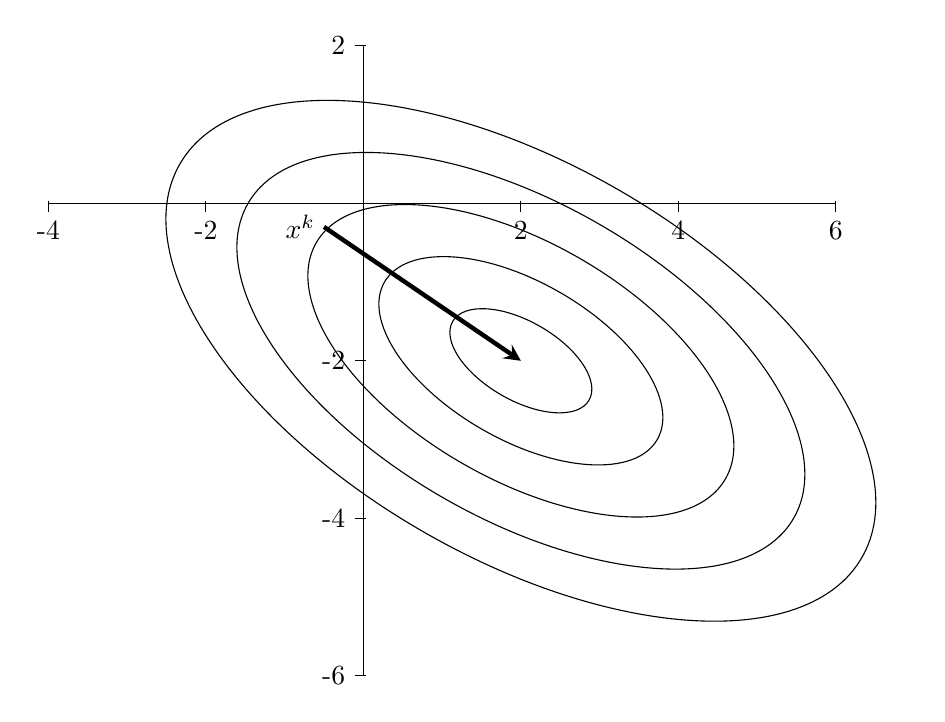
\begin{tikzpicture}
%  \begin{axis}[
%       title={Test Axis},
%       xlabel={Test X Label},
%       ylabel={Test Y Label},
%     ]
%  \end{axis}
 \draw (-4,0) -- (6,0);
 \draw (0,-6) -- (0,2);

 \foreach \x in {-4,-2,2,4,6}
   \draw (\x,1pt) -- (\x,-3pt) node[anchor=north] {\x};
 \foreach \y in {-6,-4,-2,2}
   \draw (1pt,\y) -- (-3pt,\y) node[anchor=east] {\y};

 \draw (2,-2) ellipse [x radius=1cm,y radius=0.5cm,rotate=-30];
 \draw (2,-2) ellipse [x radius=2cm,y radius=1.0cm,rotate=-30];
 \draw (2,-2) ellipse [x radius=3cm,y radius=1.5cm,rotate=-30];
 \draw (2,-2) ellipse [x radius=4cm,y radius=2.0cm,rotate=-30];
 \draw (2,-2) ellipse [x radius=5cm,y radius=2.5cm,rotate=-30];

 \node at (-0.8,-0.3) {$x^k$};
 \draw [ultra thick,-stealth] (-0.5,-0.3) -- (2,-2);

\end{tikzpicture}
\end{center}

Allgemeiner: $e^k$ ist Linearkombination von Eigenvektoren.

Sei $\lbrace v_j \rbrace$ Orthonormalbasis von Eigenvektoren
\begin{align*}
 e^k & =\sum_{j=1}^n \xi_jv_j.
\end{align*}
(Zur Einfachheit lassen wir das $k$ weg.)

Wir erhalten:
\begin{align*}
 r^Tr
 & =
 (-Ae)^T (-Ae) = \bigg(A \sum_i \xi_iv_i \bigg)^T \bigg(A \sum_j \xi_jv_j \bigg) \\
 & = \bigg(\sum_i \xi_i \lambda_iv_i \bigg)^T \bigg(\sum_j \xi_j \lambda_jv_j \bigg)=\sum_j \xi_j^2 \lambda_j^2.
\end{align*}
Ebenso:
\begin{align*}
 r^TAr & =\sum_j \xi_j^2 \lambda_j^3
\end{align*}
Der nächste Fehler ist damit
\begin{align*}
 e^{k+1}
 & =
 e^k+\frac{r_k^Tr_k}{r_k^TAr_k}r_k
 =
 e^k+\frac{\sum_j \xi_j^2 \lambda_j^2}{\sum_j \xi_j^2 \lambda_j^3} r_k.
\end{align*}

\emph{Beachte:} Falls alle $\lambda_j$ gleich sind, so sind wir wieder in einem Schritt fertig, da dann $r_k=-\lambda e^k$.

Anschauung dazu: Das Funktional ist dann kugelsymmetrisch.

\bigskip

Der folgende Satz beschreibt den allgemeinen Fall.  Den Beweis findet man bei \citet{shewchuk:1994}.

\begin{satz}[{\cite[Kapitel~6]{shewchuk:1994}}]
Sei $\kappa$ die Kondition der Matrix $A$. Dann gilt nach $k$ Schritten des Gradientenverfahrens
\begin{equation*}
 \norm{e^k}_A \leq \Big(\frac{\kappa-1}{\kappa+1}\Big)^k \norm{e^0}_A,
\end{equation*}
wobei $\norm{\cdot}_A$ die Energienorm ist.
\end{satz}

\section{Das Verfahren der konjugierten Gradienten (CG)}

(Ursprünglich vorgestellt von Hestenes und Stiefel im Jahr 1952~\cite{hestenes_stiefel:1952})

Wir halten fest:
\begin{itemize}
 \item Das Gradientenverfahren minimiert häufig mehrfach in ähnliche Richtungen.
\end{itemize}

Besser wäre doch:
\begin{enumerate}
 \item $n$ orthogonale Suchrichtungen $d_1,\ldots,d_n$
 \item Bei jedem Schritt könnten wir die richtige Schrittweite $\alpha^k$ bestimmen.
\end{enumerate}
Damit hätten wir die exakte Lösung nach $n$ Schritten.

\bigskip

\emph{Problem:} 2) heißt gerade: $e^{k+1}$ muss senkrecht auf der Suchrichtung $d_k$ stehen.

Bestimme $\alpha$:
\begin{equation*}
 0 = d_k^Te^{k+1} = d_k^T (e^k+\alpha^kd_k ) \iff \alpha^k=-\frac{d_k^Te^k}{d_k^Td_k}.
\end{equation*}
\definecolor{darkgreen}{rgb}{0,.5,0}
Geht nicht, denn $e^k$ ist unbekannt!

\medskip

Stattdessen: \emph{Gute Idee Nr.~1:} Wähle stattdessen $A$-orthogonale Suchrichtungen
(auch \emph{konjugierte} Suchrichtungen).

\medskip

Bestimme $\alpha^k$ so, dass $d_k$ und $e^{k+1}$ $A$-orthogonal sind:
\begin{align*}
 d_k^TAe^{k+1}
 & =
 d_k^TA(e^k+ \alpha^kd_k) = 0 \\
 \implies & \alpha^k=-\frac{d_k^TAe^k}{d_k^TAd_k}=\frac{d_k^T \textcolor{darkgreen}{r_k}}{d_k^TAd_k}.
\end{align*}
Dabei haben wir benutzt dass
\begin{equation*}
 r_k
 =
 b-Ax^k
 =
 A(A^{-1}b - x^k)
 =
 A(x^* - x^k)
 =
 -Ae^k.
\end{equation*}



\begin{lemma}
Auch mit $A$-orthogonalen Suchrichtungen ist man nach $n$ Schritten fertig.
\end{lemma}
\begin{proof}
Schreibe Anfangsfehler $e^0$ als Linearkombination der Suchrichtungen
\begin{equation}
\label{equa:eqerror1}
 e^0=\sum_{j=1}^{n} \delta_jd_j.
\end{equation}
Gesucht ist eine Formel für $\delta_k$. Multipliziere \eqref{equa:eqerror1} mit $d_k^TA$. Man erhält
\begin{align*}
 d_k^TAe^0 & =\sum_{j=1}^n \delta_jd_k^TAd_j=\delta_kd_k^TAd_k \\
 %
 \implies \delta_k & =\frac{d_k^TAe^0}{d_k^TAd_k}
  =
  \frac{d_k^TA \big(e^0+\sum_{i=1}^{k-1} \alpha^id_i \big)}{d_k^TAd_k} \\
 & =
 \frac{d_k^TAe^k}{d_k^TAd_k}=-\alpha^k.
\end{align*}
Bei jedem Schritt wird genau ein Summand aus der Fehlerdarstellung \eqref{equa:eqerror1} entfernt.

$\implies$ fertig nach $n$ Schritten, da dann $e^n=0$.
\end{proof}

\subsection{Das Gram-Schmidt-Verfahren}

Wie erzeugt man $A$-orthogonale Richtungen?

\medskip

Wir erklären jetzt, wie man $n$ $A$-orthogonale Suchrichtungen konstruieren kann.
Im CG-Verfahren passiert das synchron zum eigentlichen Suchen des Minimierers.
Es wird \emph{nicht} zuerst die Menge der Suchrichtungen konstruiert, und dann
erst eine nach der anderen zur Suche genommen.

\begin{itemize}
 \item Seien $u_1,\ldots,u_n$ linear unabhängige Vektoren.
 \item Setze:
  \begin{equation}
    \label{equa:eqschmidt1}
   d_i=u_i+\sum_{j=1}^{i-1} \beta_{ij}d_j, \qquad \qquad \beta_{ij}=-\frac{u_i^TAd_j}{d_j^TAd_j}.
  \end{equation}
\end{itemize}
Funktioniert, aber:
\begin{enumerate}
 \item Man muss sich alle $d_j$ merken $\longrightarrow \mathcal{O} (n^2)$ Speicherverbrauch
 \item Benötigt $\mathcal{O} (n^3)$ Rechenoperationen.  Das ist in etwa so viel wie
   wie bei Gauß-Elimination, also zu viel.
\end{enumerate}

\subsection{Das Verfahren der konjugierten Gradienten}

(Eigentlich ein schlechter Name: Es kommen keine konjugierten Gradienten vor.)

\bigskip

\emph{Gute Idee Nr.~2:} Wähle $u_i=r^i$ für $i=1,\ldots,n$.
\begin{itemize}
\item Warum ist das eine gute Idee?
\item Geht das überhaupt?
\item Bilden die $r^i$ eine linear unabhängige Menge?
\end{itemize}

\emph{Bemerkung:} Wie kann das gehen?  Zum Berechnen der Residuen $r^i$ brauchen wir die
Suchrichtungen, und jetzt sollen wir umgekehrt die Residuen zur Berechnung der Suchrichtungen
brauchen?  Der Trick: Wir berechnen beide abwechselnd.  Aus der Startiterierten $x^0$ folgt
das erste Residuum.  Damit kann die erste Suchrichtung berechnet werden.  Damit berechnen
wir $x^1$ und damit das zweite Residuum.  Damit dann die nächste Richung usw.

\begin{lemma}
$d_l^Tr_i=0$ für alle $l<i$.
\end{lemma}
\begin{proof}
Es gilt
\begin{align*}
 e^i & =e^0+\sum_{j=0}^{i-1} \alpha^jd_j=\sum_{j=0}^n \delta_jd_j-\sum_{j=0}^{i-1} \delta_jd_j=\sum_{j=i}^{n} \delta_jd_j.
\end{align*}
Multipliziere beide Seiten mit $-d_l^TA$:
\begin{align*}
 -d_l^TAe^i & =-\sum_{j=i}^n \delta_jd_l^TAd_j.
\end{align*}
Die linke Seite ist $d_l^T r^i$.

Die rechte Seite ist $0$, da die $d_i$ $A$-orthogonal sind.
\end{proof}


\bigskip

Nicht nur ist $r^i$ orthogonal zu allen Suchrichtungen $d_l$ mit $l<i$, es ist auch senkrecht
auf allen Residuen $r^l$ mit $l<i$!  Deshalb bilden die $r_k$ eine linear unabhängige Menge;
das Gram-Schmidt-Verfahren kann also angewandt werden.

\begin{lemma}
\label{lem:orthogonal_residuals}
$r^i$ ist orthogonal zu $r^l$ falls $l<i$.
\end{lemma}
\begin{proof}
Gram-Schmidt-Formel
\begin{equation*}
 d_l=r^l+\sum_{k=0}^{l-1} \beta_{lk}d_k.
\end{equation*}
Multipliziere von rechts mit $r^i$:
\begin{equation*}
 \underbrace{d_l^Tr^i}_{=0}
 =
 (r^l)^T r^i+\sum_{k=0}^{l-1} \beta_{lk} \underbrace{d_k^Tr^i}_{=0}.
\end{equation*}
Es folgt
\begin{equation*}
 (r^l)^T r^i = 0.
\end{equation*}
Die Residuen $r^1,\ldots,r^n$ sind linear unabhängig.
\end{proof}

Es passiert etwas magisches!
\begin{lemma}
Fast alle $\beta_{ij}$ verschwinden! Gram-Schmidt wird billig.
\end{lemma}
\begin{proof}
\begin{itemize}
 \item $r^{j+1}=-Ae^{j+1}=-A (e^j+\alpha^jd_j)=r^j-\alpha^jAd_j$

 \item Multipliziere von links mit $r_i^T$
  \begin{align*}
   \alpha^j (r_i^TAd_j) & =\underbrace{r_i^Tr_j}_{=0 \thinspace \Leftarrow \thinspace i \neq j}
      -\underbrace{r_i^Tr_{j+1}}_{=0 \thinspace \Leftarrow \thinspace i \neq j+1}
  \end{align*}
 Wegen Lemma~\ref{lem:orthogonal_residuals} ist der Term auf der rechten Seite
 fast immer Null!  Genauer:
  \begin{align*}
   r_i^TAd_j
    & =
    \begin{cases}
      \frac{1}{\alpha^i} (r^i)^Tr^i &  \text{falls $i=j$,} \\
     -\frac{1}{\alpha^{i-1}} (r^i)^T r^i & \text{falls $i=j+1$,} \\
     0 & \text{sonst.}
    \end{cases}
  \end{align*}

 \item Gram-Schmidt-Koeffizienten:
  \begin{equation*}
   \beta_{ij}
    =
   -\frac{(r^i)^TAd_j}{d_j^TAd_j}
    =
   \begin{cases}
   \frac{1}{\alpha^{i-1}} \frac{\left(r^i \right)^T r^i}{d_j^TAd_j} & \text{falls $i=j+1$,} \\
     0 &  \text{sonst}.
   \end{cases}
  \end{equation*}
  Der Fall $i=j$ tritt im Gram-Schmidt-Verfahren nicht auf! \qedhere
\end{itemize}
\end{proof}
Formel \eqref{equa:eqschmidt1} reduziert sich:
\begin{equation}
\label{eq:simplified_gram_schmidt_coefficient}
 \text{Aus}
 \qquad d_i=u_i+\sum_{j=1}^{i-1} \beta_{ij}d_j
 \qquad \text{wird}
 \qquad d_i=u_i+\beta_{i,i-1}d_{i-1}.
\end{equation}
\begin{itemize}
 \item Fast alle $\beta_{ij}$ sind Null!
 \item Deshalb: Einfachere Notation: Schreibe $\beta_{(i)}$ statt $\beta_{i,i-1}$.
 \item Es werden nicht mehr alle $d_i$ benötigt, um die nächste Richtung auszurechnen.
 \item Speicheraufwand und Rechenzeit geht von $\mathcal{O} \left(n^2 \right)$ nach $\mathcal{O}(n \cdot$ Anzahl der Einträge von $A)$.
\end{itemize}

Wir können die Darstellung von $\beta_{(i)}$ noch weiter vereinfachen.
\begin{itemize}
 \item Setze zunächst $\alpha^i=\frac{d_i^Tr^i}{d_i^TAd_i}$ in die Definition von $\beta_{i,i-1}$ ein.
  Man erhält
  \begin{equation*}
   \beta_{(i)}=\frac{(r^i)^Tr^i}{d_{i-1}^Tr_{i-1}}
  \end{equation*}
 %
 \item Aus~\eqref{eq:simplified_gram_schmidt_coefficient} folgt
 \begin{equation*}
  d^T_{i-1}r_{i-1}
  =
  u^T_{i-1} r_{i-1} + \beta_{i-1,i-2} \underbrace{d^T_{i-2}r_{i-1}}_{=0}
  =
  u^T_{i-1} r_{i-1}
  =
  r^T_{i-1} r_{i-1}.
 \end{equation*}
 %
 \item Damit erhält man
  \begin{equation*}
   \beta_{(i)} = \frac{(r^i)^Tr^i}{r_{i-1}^Tr_{i-1}}.
  \end{equation*}

\end{itemize}



\subsection{Das komplette Verfahren}
\begin{itemize}
 \item Berechne $d_0=r_0=b-Ax^0$.
 \item Für $k=1,2,3,\ldots$
   \begin{align*}
    \alpha^k & =\frac{r_k^Tr_k}{d_k^TAd_k} \\
    x^{k+1} & =x^k+\alpha^kd^k \\
    r^{k+1} & =b-Ax^{k+1}=r_k-\alpha^kAd_k \\
    \beta_{(k+1)} & =\frac{r_{k+1}^Tr_{k+1}}{r_k^Tr_k} \\
    d_{k+1} & =r_{k+1}+\beta_{(k+1)}d_k
   \end{align*}
\end{itemize}
Direkter Löser mit Komplexität $\mathcal{O}(n \cdot$ Anzahl der Einträge von $A)$. Einige Fakten zu CG \begin{itemize}
	\item Zuerst vorgeschlagen von Magnus Hestenes und Eduard Stiefel im Jahr 1952
	\item Toll: ein direkter Löser für dünnbesetzte lineare GS mit Komplexität $\mathcal{O}(n \cdot$ Anzahl der Einträge von $A)$.
	\item Funktioniert in der Praxis aber schlecht: Rundungsfehler zerstören $A$-Orthogonalität der Richtungen, man hat nach $n$ Iterationen also \emph{nicht} die Lösung
	\item Geriet zwischenzeitlich in Vergessenheit
	\item Erlebte Revival als iterative Methode
\end{itemize}

\subsection{Interpretation als Krylov-Verfahren}
CG hat weitere interessante Eigenschaften.

Die Folge der Suchrichtungen $d_0, d_1, \dots$ definiert eine Folge von Räumen
\begin{align*}
 \D_0 & =\spann \{d_0\} \\
 \D_1 & =\spann \{d_0,d_1\} \\
 \D_2 & =\spann \{d_0,d_1,d_2\} \\
 & \vdots
\end{align*}
\begin{satz}
Das CG-Verfahren wählt $x_k$ so aus dem Raum $e_0+\D_k$, dass $\norm{e_k}_A$ minimal ist.
\end{satz}

[Dies ist auch eine alternative Motivation des Verfahrens.]

\bigskip

Alternative Charakterisierung der $\D_k$
\begin{align*}
	\D_k & =\spann \left\lbrace d_0,Ad_0,A^2d_0,\ldots,A^kd_0 \right\rbrace \\
	& =\spann \left\lbrace r_0,Ar_0,A^2r_0,\ldots,A^kr_0 \right\rbrace.
\end{align*}

\begin{itemize}
 \item Solche Räume heißen \emph{Krylov-Räume}.\footnote{Nach Alexei Nikolajew Krylow, 1863-1945}
 %
 \item CG heißt deshalb auch ein "`Krylov-Verfahren"'.
 %
 \item Es gibt noch weitere Krylov-Raum-basierte Verfahren, z.B. BiCGStab, MinRes, GMRes.
\end{itemize}

\subsection{Konvergenz des CG-Verfahren als iterativem Verfahren}
\begin{satz}
Für alle $k=1,\ldots,n$ hat der Fehler $e^k$ die Darstellung
\begin{equation*}
 e^k=\bigg(I+\sum_{j=1}^k \psi_jA^j \bigg)e^0,
\end{equation*}
wobei die Koeffizienten $\psi_1,\ldots,\psi_k \in \R$ von $\alpha^i$ und $\beta_{(i)}$ für $i=1,\ldots,k$ abhängen.
\end{satz}

\paragraph*{Hauptidee:}
\begin{itemize}
 \item CG minimiert $\Vert e_k \Vert_A$
 \item Der Ausdruck in der Klammer ist ein Polynom in $A$, also
  \begin{equation*}
   e^k=P_k(A)e^0
  \end{equation*}

 \item Interpretation von CG:
  \begin{enumerate}
   \item CG wählt die Koeffizienten $\alpha_i,\beta_{(i)}$
   \item CG konstruiert das Polynom $P_k(A)$
  \end{enumerate}
\end{itemize}

\bigskip

Wie wirkt $P_k(A)$ auf $e^0$?
\begin{itemize}
 \item Schreibe $e^0$ in orthonormaler Eigenvektor-Basis
 \begin{align*}
   e^0 & =\sum_{j=i}^n \xi_jv_j
 \end{align*}
 \item Daraus folgt
 \begin{align*}
   e^k & = \left(I+\sum_{i=1}^k \psi_iA^i \right) \sum_{j=1}^n \xi_jv_j \\
   & = \sum_{j=1}^n \xi_j \left(I+\sum_{i=1}^k \psi_iA^i \right)v_j \\
   & = \sum_{j=1}^n \xi_j \left(1+\sum_{i=1}^k \psi_i \lambda_j^i \right)v_j \\
   & = \sum_{j=1}^n \xi_jP_k (\lambda_j)v_j
 \end{align*}
 \item Multiplikation von links mit $A$
 \begin{align*}
   Ae_k & = \sum_{j=1}^n \xi_jP_k (\lambda_j) \lambda_jv_j \\
   \norm{e_k}_A^2
   & =
   e_k^T (Ae_k)
   =
   \bigg(\sum_{i=1}^n \xi_iP_k (\lambda_i)v_i\bigg)
   \bigg(\sum_{j=1}^n \xi_jP_k (\lambda_j) \lambda_jv_j\bigg)
   =
   \sum_{j=1}^n \xi_j^2 \left(P_k \left( \lambda_j \right) \right)^2 \lambda_j
 \end{align*}
 %
 \item Das CG-Verfahren minimiert also
  \begin{align*}
   \norm{e_k}_A^2 & = \min_{\tilde{P}_k,\tilde{P}_k(0)=1} \sum_{j=1}^n \xi_j^2 \tilde{P}_k (\lambda_j)^2 \lambda_j \\
   & \leq
   \min_{\tilde{P}_k,\tilde{P}_k(0)=1} \max_{\lambda \in \sigma (A)} (\tilde{P}_k (\lambda))^2
       \underbrace{\sum_{j=1}^n \xi_j^2 \lambda_j}_{\norm{e^0}_A^2}
  \end{align*}
  Dabei ist $\sigma(A)$ das \emph{Spektrum} von $A$, d.h.\ die Menge aller Eigenwerte.
\end{itemize}
Die Aufgabe lautet also:
\begin{itemize}
 \item Finde Polynom $P_k$ mit $P_k(0)=1$, dessen Werte für Eigenwerte $\lambda$ möglichst klein sind.
\end{itemize}

\bigskip

\begin{bsp}
$A \in \R^{2 \times 2}$ mit $\sigma(A) =\lbrace 2,7 \rbrace$, also $\lambda_1=2,\lambda_2=7$.

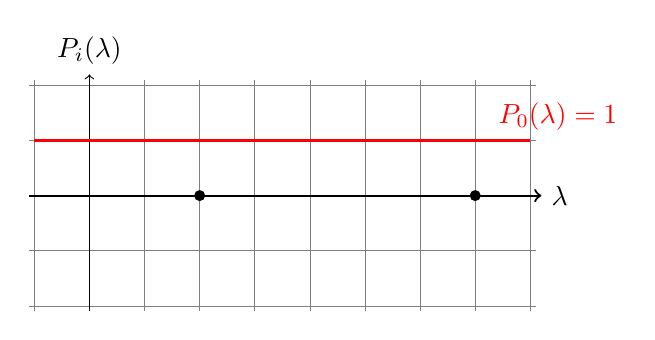
\begin{tikzpicture}[domain=-1:8,scale=0.7]
	\draw[very thin,color=gray] (-1.1,-2.1) grid (8.1,2.1);
	\draw[thick,->]	(-1.1,0) -- (8.2,0)	node[right]	{$\lambda$};
	\draw[->]	(0,-2.1) -- (0,2.2)	node[above]	{$P_i(\lambda)$};
	\draw[thick,color=red] plot (\x,1)	node[above]	{$\qquad P_0 (\lambda)=1$};
	\fill (2,0) circle [radius=0.1cm];
	\fill (7,0) circle [radius=0.1cm];
\end{tikzpicture}
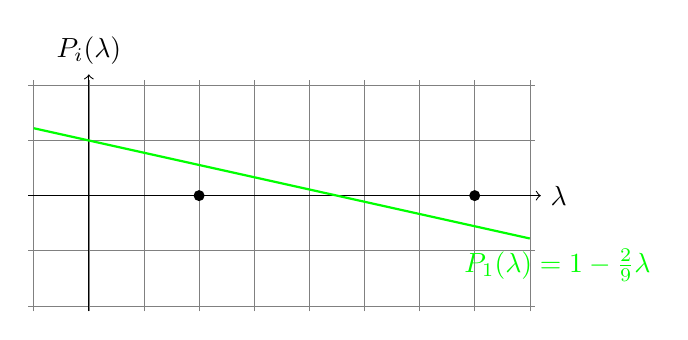
\begin{tikzpicture}[domain=-1:8,scale=0.7]
	\draw[very thin,color=gray] (-1.1,-2.1) grid (8.1,2.1);
	\draw[->]	(-1.1,0) -- (8.2,0)					node[right]	{$\lambda$};
	\draw[->]	(0,-2.1) -- (0,2.2)					node[above]	{$P_i(\lambda)$};
	\draw[thick,color=green]	plot (\x,{1-0.22222222*\x})	node[below] {$\qquad P_1(\lambda) =1-\frac{2}{9} \lambda$};
	\fill (2,0) circle [radius=0.1cm];
	\fill (7,0) circle [radius=0.1cm];
\end{tikzpicture}

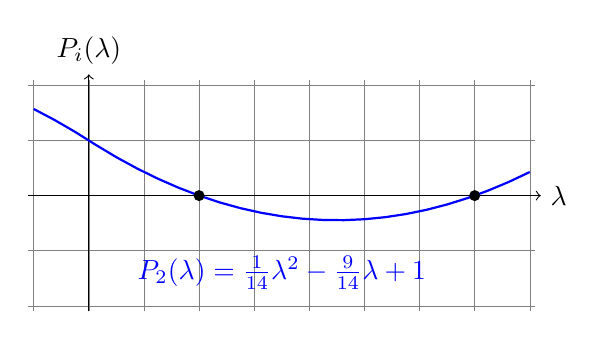
\begin{tikzpicture}[domain=-1:8,scale=0.7]
	\draw[very thin,color=gray] (-1.1,-2.1) grid (8.1,2.1);
	\draw[->]	(-1.1,0) -- (8.2,0)					node[right]	{$\lambda$};
	\draw[->]	(0,-2.1) -- (0,2.2)					node[above]	{$P_i(\lambda)$};
	\draw[thick,color=blue]	plot (\x,{0.07142857*\x^2-0.64285714*\x+1});
        \node [color=blue] at (3,-1.4) {$\qquad P_2(\lambda) = \frac{1}{14} \lambda^2-\frac{9}{14} \lambda+1$};
	\fill (2,0) circle [radius=0.1cm];
	\fill (7,0) circle [radius=0.1cm];
\end{tikzpicture}
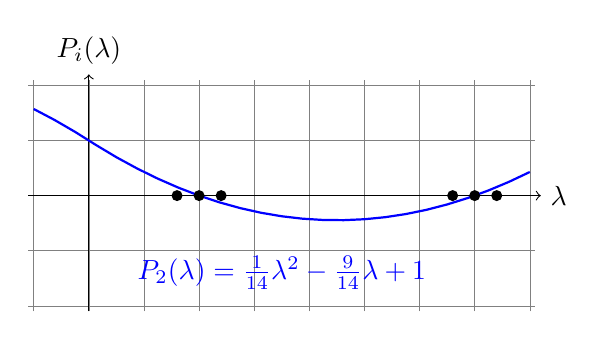
\begin{tikzpicture}[domain=-1:8,scale=0.7]
	\draw[very thin,color=gray] (-1.1,-2.1) grid (8.1,2.1);
	\draw[->]	(-1.1,0) -- (8.2,0)					node[right]	{$\lambda$};
	\draw[->]	(0,-2.1) -- (0,2.2)					node[above]	{$P_i(\lambda)$};
	\draw[thick,color=blue]	plot (\x,{0.07142857*\x^2-0.64285714*\x+1});
	\node [color=blue] at (3,-1.4) {$\qquad P_2(\lambda) = \frac{1}{14} \lambda^2-\frac{9}{14} \lambda+1$};
	\foreach \x in {1.6,2,2.4, 6.6,7,7.4}
	  \fill (\x,0) circle [radius=0.1cm];
\end{tikzpicture}

Schnelle Konvergenz, wenn
\begin{itemize}
 \item es ein Polynom niedrigen Grades gibt, dass bei allen Eigenwerten von $A$ niedrige Werte annimmt.
 \item Eigenwerte von $A$ in Haufen auftreten
 \item viele Eigenwerte mehrfach auftreten
\end{itemize}


Schlimmst-möglicher Fall:
\begin{itemize}
	\item Eigenwerte sind gleichverteilt in $\left[\lambda_{\min},\lambda_{\max} \right]$.
	\item Wenig doppelte Eigenwerte.
\end{itemize}

\bigskip

Allgemein ist zuwenig über die Eigenwerte von $A$ bekannt.

\end{bsp}
\emph{Ansatz}: Anstelle das Maximum von $P_k$ über alle Eigenwerte von $A$ zu minimieren,
minimieren wir das Maximum von $P_k$ auf ganz $\left[\lambda_{\min},\lambda_{\max} \right]$.
\begin{align*}
 \norm{e^k}_A^2
  & \leq
 \min_{\tilde{P}_k,\tilde{P}_k(0)=1} \max_{\lambda \in [\lambda_{\min},\lambda_{\max}]}
     (\tilde{P}_k(\lambda ))^2 \norm{e^0}_A^2
\end{align*}
\begin{defi}
Das Tschebyshew-Polynom vom Grad $i \in \N$ ist
\begin{equation*}
 T_i(s)=\frac{1}{2} \Big[ (s+\sqrt{s^2+1})^i + (s-\sqrt{s^2-1} )^i \Big].
\end{equation*}
\end{defi}
\begin{satz}
Es gilt
\begin{equation*}
 \abs{T_i(s)} \leq 1
 \qquad
 \text{für alle $s \in [-1,1]$},
\end{equation*}
und $T_i$ ist "`maximal außerhalb von $[-1,1]$"' unter allen Polynomen mit dieser Eigenschaft.
\end{satz}
Umskalieren:
\begin{lemma}
Das Polynom
\begin{equation*}
 \tilde{T}_i(\lambda)
 =
 \frac{T_i \left( \frac{\lambda_{\max}+\lambda_{\min}-2 \lambda}{\lambda_{\max}-\lambda_{\min}} \right)}{T_i \left(\frac{\lambda_{\max}+\lambda_{\min}}{\lambda_{\max}-\lambda_{\min}} \right)}
\end{equation*}
oszilliert auf $[\lambda_{\min},\lambda_{\max}]$ zwischen
\begin{equation*}
 \pm T_i \left( \frac{\lambda_{\max}+\lambda_{\min}}{\lambda_{\max}-\lambda_{\min}} \right)^{-1},
\end{equation*}
und erfüllt $\tilde{T}_i(0)=1$.
\end{lemma}
Damit können wir den Fehler abschätzen:
\begin{align*}
 \norm{e^k}_A
 & \leq
 \min_{\tilde{P}_k,\tilde{P}_k(0)=1} \max_{\lambda \in [ \lambda_{\min},\lambda_{\max}]}
     \abs{P_k(\lambda)} \cdot \norm{e^0}_A \\
 & \leq
 \max_{\lambda \in [\lambda_{\min},\lambda_{\max}]} \abs{\tilde{T}_k (\lambda)} \cdot \norm{e^0}_A \\
 & \leq
 T_i \left(\frac{\lambda_{\max}+\lambda_{\min}}{\lambda_{\max}-\lambda_{\min}} \right)^{-1} \cdot \norm{e^0}_A
\end{align*}
Da $A$ s.p.d.\ ist gilt $\kappa = \kappa(A) = \frac{\abs{\lambda_\text{max}}}{\abs{\lambda_\text{min}}}
  = \frac{\lambda_\text{max}}{\lambda_\text{min}}$, und deshalb
\begin{align*}
 \norm{e^k}_A
 & =
 T_i \left(\frac{\kappa +1}{\kappa -1} \right)^{-1} \norm{e^0}_A \\
 & =
 2 \left[ \left( \frac{\sqrt{\kappa}+1}{\sqrt{\kappa}-1} \right)^k
         +\left( \frac{\sqrt{\kappa}-1}{\sqrt{\kappa}+1} \right)^k \right]^{-1} \cdot \norm{e^0}_A
\end{align*}
Der zweite Summand geht gegen $0$ für $k \to \infty$.  Deshalb
\begin{align*}
 \norm{e^k}_A \leq 2 \left( \frac{\sqrt{\kappa}-1}{\sqrt{\kappa}+1} \right)^k \cdot \norm{e^0}_A
\end{align*}
\begin{itemize}
 \item Vergleiche mit Gradientenverfahren. Dort:
  \begin{equation*}
   \norm{e^k}_A \leq \left(\frac{\kappa -1}{\kappa +1} \right)^k \norm{e^0}_A
  \end{equation*}
 %
 \item Das ist langsamer als für das CG-Verfahren.
 %
 \item Diese Abschätzung für CG ist aber sehr schwach. In vielen Fällen konvergiert das Verfahren deutlich besser!
\end{itemize}


\section{Vorkonditionierung}

Die Konvergenzrate von CG (und diversen anderen Verfahren) hängt von der Kondition von $A$ ab.

\subsection{Idee der Vorkonditionierung}

Wähle eine Matrix $W$, die $A$ "`gut approximiert"', und betrachte das Gleichungssystem
\begin{equation*}
 W^{-1}Ax=W^{-1}b.
\end{equation*}

\begin{itemize}
 \item Gleiche Lösung wie $Ax=b$.
 \item Bei geschickt gewähltem $W$ ist $\kappa \left(W^{-1}A \right) \ll \kappa (A)$
\end{itemize}
Löse $W^{-1}Ax=W^{-1}b$ mit dem CG-Verfahren.

\medskip

\emph{Problem}: Das CG-Verfahren kann nur verwendet werden, wenn $W^{-1}A$ s.p.d.\ ist,\\
 aber aus $W$ und $A$ s.p.d. folgt \emph{nicht}, dass $W^{-1}A$ s.p.d. ist.

\medskip

\emph{Trick}: Wähle $W$ s.p.d.

Dann existiert die Cholesky-Zerlegung
\begin{equation*}
 W=L_1L_1^T=LDL^T
\end{equation*}
mit
\begin{itemize}
 \item $D$ Diagonalmatrix
 \item $L$ untere Dreiecksmatrix mit Einsen auf der Diagonalen
 \item $L_1=LD^{\frac{1}{2}}$ untere Dreiecksmatrix
\end{itemize}
Statt $Ax=b$ betrachte
\begin{equation*}
 \underbrace{L_1^{-1}AL_1^{-T}}_{\equalscolon \tilde{A}} \underbrace{L_1^Tx}_{\equalscolon\tilde{x}}
 =
 \underbrace{L_1^{-1}b}_{\equalscolon\tilde{b}}
\end{equation*}
also
\begin{equation*}
 \tilde{A} \tilde{x} = \tilde{b}.
\end{equation*}

Die neue Matrix $\tilde{A}$ ist s.p.d., es gilt sogar:

\begin{satz}
$W^{-1}A$ und $\tilde{A} = L_1^{-1}AL_1^{-T}$ haben die gleichen Eigenwerte.
\end{satz}
\begin{proof}
Sei $v$ Eigenvektor von $W^{-1}A$, dann ist $L_1^Tv$ Eigenvektor von $\tilde{A}$ zum selben Eigenwert.
\end{proof}

Da $\tilde{A}$ s.p.d.\ ist können wir CG verwendet werden:
\begin{equation*}
 \tilde{d}_0
 =
 \tilde{r}^0
 =
 \tilde{b}-\tilde{A} \tilde{x}^0
 =
 L_1^{-1}b-L_1^{-1}AL_1^{-T} \tilde{x}^0
 =
 L_1^{-1} (b-Ax^0)
\end{equation*}
Für $k=1,2,3,\ldots$
\begin{align*}
 \alpha^k & =\frac{\tilde{r}_k^T \tilde{r}_k}{\tilde{d}_kL_1^{-1}A L_1^{-T} \tilde{d}_k} \\
 \tilde{x}^{k+1} & =\tilde{x}^k+\alpha^k \tilde{d}_k \\
 \tilde{r}_{k+1} & =\tilde{r}_k-\alpha^k L_1^{-1}AL_1^{-T} \tilde{d}_k \\
 \beta_{(k+1)} & =\frac{\tilde{r}_{k+1}^T \tilde{r}_{k+1}}{\tilde{r}_k^T \tilde{r}_k} \\
 \tilde{d}_{k+1} & =\tilde{r}_{k+1}+\beta_{(k+1)} \tilde{d}_k
\end{align*}
Zu teuer: $L_1$ muss bekannt sein!

\bigskip

Stattdessen: Setze $d_k=L_1^{-T} \tilde{d}_k$.

Das umgeformte Verfahren ist:
\begin{align*}
 d_0 & = L_1^{-T} \tilde{d}_0 = L_1^{-T}L_1^{-1} (b-Ax^0)=W^{-1}r_0
\end{align*}
Für $k=1,2,3,\ldots$
\begin{align*}
 \alpha^k & =\frac{r_k^T W^{-1} r_k}{d_k^TAd_k} \\
 x^{k+1} & =x^k+\alpha^kd^k \\
 r_{k+1} & = r_k-\alpha^kAd_k \\
 \beta_{(k+1)} & =\frac{r_{k+1}^T W^{-1} r_{k+1}}{r_k^TW^{-1}r_k} \\
 d_{k+1} & =W^{-1}r_{k+1}+\beta_{(k+1)}d_k
\end{align*}
Mit einem Wort: Wir nehmen ersetzen im normalen CG-Verfahren einfach überall $r$ durch $W^{-1}r$.


Dieses Verfahren heißt \emph{Vorkonditioniertes CG-Verfahren}. Es funktioniert gut, wenn
\begin{enumerate}
 \item $\kappa \left(W^{-1}A \right)$ klein ist
 \item Die Lösung von $Wz=r_k$ billig berechnet werden kann.
\end{enumerate}


\subsection{Unvollständige Cholesky-Zerlegung (ICH,ILU,\ldots)}

Für die Wahl von $W$ sind extrem viele verschiedene Möglichkeiten vorgeschlagen worden.

\medskip

Wir zeigen zwei wichtige Ansätze.

\medskip

\emph{Idee:} Die beste Kondition bekäme man natürlich für $W=A$.

Zur Lösung von $Wz=Az=r_k$ Cholesky-Zerlegung $A=LDL^T$ berechnen \\
(viele GS mit fester Matrix).
\begin{itemize}
 \item Selbst für dünnbesetzte $A$ ist $L$ aber vollbesetzt \newline
 $\implies$ Lösen mit Cholesky-Zerlegung ist zu teuer und braucht zu viel Speicher.
\end{itemize}

\begin{defi}
Sei $A \in \R^{n \times n}$ symmetrisch und positiv definit. Eine unvollständige Cholesky-Zerlegung von $A$ ist
$A \approx \tilde{L} \tilde{D} \tilde{L}^T$, wobei
\begin{itemize}
 \item $\tilde{L}$ : normierte untere Dreiecksmatrix
 \item $\tilde{D}$ : Diagonalmatrix
 \item $\tilde{L}_{ij}=0$ falls $A_{ij}=0$
\end{itemize}
\end{defi}

\bigskip

Vorkonditionierer: $W=\tilde{L} \tilde{D} \tilde{L}^T$
\begin{itemize}
 \item häufig: $\kappa \left(W^{-1}A \right) \ll \kappa (A)$
 \item $\tilde{L}$ ist dünnbesetzt: $\implies \tilde{L} \tilde{D} \tilde{L}^Tz^k=r_k$ ist billig zu lösen.
\end{itemize}


\subsubsection{Konstruktion der unvollständigen Cholesky-Zerlegung}

Statt $\tilde{L} \tilde{D} \tilde{L}^T$ berechnen wir $\tilde{L} \tilde{R}$.

\smallskip

Dann ist nämlich $\tilde{R} = \tilde{D} \tilde{L}^T$ mit $\tilde{D} = \operatorname{diag} \tilde{R}$.

\bigskip

Sei $A=LR$ mit $L$, $R$ Dreiecksmatrizen, $L$ normiert.

Dann ist
\begin{align*}
 A_{ik} & =\sum_{j=1}^n L_{ij}R_{jk}
    = \sum_{j=1}^i L_{ij}R_{jk}
    = \underbrace{L_{ii}}_{=1} R_{ik}+\sum_{j=1}^{i-1} L_{ij}R_{jk}
\end{align*}
Damit kann man den Eintrag $R_{ik}$ berechnen:
\begin{align*}
 R_{ik} & =A_{ik}-\sum_{j=1}^{i-1} L_{ij}R_{jk}
 \qquad
 \text{da $L_{ii}= 1$}, \quad
 1 \leq i<k \leq n
\end{align*}
Ähnlich:
\begin{equation*}
 L_{ik}=R_{ii}^{-1} \Big(A_{ik}-\sum_{j=1}^{k-1} L_{ij}R_{jk} \Big)
 \qquad 1 \leq k<i \leq n
\end{equation*}
Mit diesen Formeln kann man eine LR-Zerlegung berechnen.

\begin{algorithm}[H]
 \SetAlgoLined
 % \caption{...}
 \SetKwInOut{Input}{input}
 \Input{$A \in \R^{n \times n}$}
 Setze $L=I \in \R^{n \times n},R=0 \in \R^{n \times n}$\\
 \For{$i = 1,2,\dots,n$}
 {
   \For{$k=1,\dots,i-1$}
   {
     $\displaystyle L_{ik} = R_{kk}^{-1} \Big( A_{ik} - \sum_{j=1}^{k-1} L_{ij} R_{jk} \Big)$
   }
   \For{$k=i,\dots,n$}
   {
     $\displaystyle R_{ik} =  A_{ik} - \sum_{j=1}^{i-1} L_{ij} R_{jk}$
   }
 }
\end{algorithm}

Um stattdessen eine \emph{unvollständige} LR-Zerlegung zu berechnen lassen wir einfach alle Einträge $i,j$ aus,
für die $A_{ij}=0$ gilt.

\medskip

\begin{algorithm}[H]
 \SetAlgoLined
 % \caption{...}
 \SetKwInOut{Input}{input}
 \Input{$A \in \R^{n \times n}$}
 Setze $\tilde{L}=I \in \R^{n \times n},\tilde{R}=0 \in \R^{n \times n}$\\
 \For{$i = 1,2,\dots,n$}
 {
   \ForEach{$k=1,\dots,i-1$ with $A_{ik} \neq 0$}
   {
     $\displaystyle \tilde{L}_{ik} = \tilde{R}_{kk}^{-1} \Big( A_{ik} - \sum_{j=1}^{k-1} \tilde{L}_{ij} \tilde{R}_{jk} \Big)$
     \qquad Summe nur über das Muster
   }
   \ForEach{$k=i,\dots,n$ with $A_{ik} \neq 0$}
   {
     $\displaystyle \tilde{R}_{ik} =  A_{ik} - \sum_{j=1}^{i-1} \tilde{L}_{ij} \tilde{R}_{jk}$
     \qquad Summe nur über das Muster
   }
 }
\end{algorithm}


\begin{bsp}
Poisson-Problem. CG vs.\ CG mit ILR-Vorkonditionierer
\begin{equation*}
\begin{tabular}{c|c|ccc}
h & $\frac{1}{40}$ & $\frac{1}{80}$ & $\frac{1}{160}$ & $\frac{1}{320}$ \\
\hline
CG & 65 & 130 & 262 & 525 \\
ILR-CG & 20 & 40 & 79 & 157
\end{tabular}
\end{equation*}
Tabelle: Anzahl der Iterationen um das Residuum um den Faktor $1000$ zu reduzieren.
\end{bsp}

Es sind viele Varianten möglich!

\subsection{Lineare Verfahren als Vorkonditionierer}
\emph{Erinnerung:} Lineares Verfahren
\begin{equation*}
 x^{k+1}=x^k+C (b-Ax^k)
\end{equation*}
Sei
\begin{enumerate}
 \item $A$ symmetrisch und positiv definit
 \item $C$ so, dass $\rho (I-CA)<1$, d.h. das Verfahren konvergiert.
\end{enumerate}
Wir hatten $C$ als Approximation von $A^{-1}$ interpretiert.

\bigskip

\emph{Idee}: Wähle $W^{-1}=C$ als Vorkonditionierer für CG.

\medskip

\emph{Praktische Umsetzung}: Für CG müssen Ausdrücke der Form $z = W^{-1} r_k = Cr_k$ berechnet werden.

\medskip

\emph{Problem}: $C$ ist i.\,A.\ nicht explizit gegeben.

\smallskip

\emph{Lösung:} Betrachte das lineare Gleichungssystem $Az=r_k$
\begin{itemize}
 \item Setze $z^0=0 \in \R^n$
 \item Ein Schritt des linearen Verfahrens:
  \begin{equation*}
   z^1=z^0+C (r_k-Az^0)=Cr_k
  \end{equation*}
\end{itemize}

\bigskip

Viele lineare Verfahren können als Vorkonditionierer verwendet werden!

\begin{itemize}
 \item Z.\,B.: Der Jacobi-Vorkonditionierer: $C=\operatorname{diag} (A)^{-1}$
 \item Viele lineare Verfahren werden überhaupt nur betrachtet, um als Vorkonditionierer zu dienen
       (z.\,B. Mehrgitterverfahren, Gebietszerlegungsverfahren).
\end{itemize}
Ein Problem noch: Wie steht es z.\,B.\ mit Gauß--Seidel
\begin{equation*}
 C = (D-L)^{-1}
 \qquad ?
\end{equation*}
\begin{itemize}
	\item Funktioniert nicht, denn $W=C^{-1}=D-L$ ist nicht symmetrisch.
\end{itemize}
\medskip
Stattdessen: Symmetrischer Gauß--Seidel
\begin{itemize}
 \item Abwechselnd
  \begin{itemize}
   \item Vorwärtsiteration:
    \begin{equation*}
     x^{k+\frac{1}{2}}=x^k+(D-L)^{-1} (b-Ax^k)
    \end{equation*}
   %
   \item Rückwärtsiteration:
    \begin{equation*}
     x^{k+1}=x^{k+\frac{1}{2}}+(D-R)^{-1} (b-Ax^{k+\frac{1}{2}})
    \end{equation*}
   \end{itemize}
 \item Einsetzen:
  \begin{equation*}
   x^{k+1}=x^k+\underbrace{\left[(D-L)^{-1}+(D-R)^{-1}-(D-R)^{-1}A(D-L)^{-1} \right]}_{=C} (b-Ax^k)
  \end{equation*}
  Dieses $C$ will man sicher nicht explizit ausrechnen.
 \item Aber: $C^{-1}=W$ ist s.p.d.!
\end{itemize}

\bigskip

Auch im linearen Verfahren selbst kann man $C$ als Vorkonditionierer interpretieren.
\begin{itemize}
 \item Lineares Gleichungssystem $Ax=b$
 \item Richardson-Verfahren
  \begin{equation*}
   x^{k+1}=x^k + (b-Ax^k)
  \end{equation*}
 \item Vorkonditionierung: Wähle ein $W$ als Approximation von $A$. Betrachte
  \begin{equation*}
   W^{-1}Ax=W^{-1}b
  \end{equation*}
  Statt $W^{-1}$ schreibe $C$:
  \begin{equation*}
   CAx=Cb
  \end{equation*}
 \item Richardson-Iteration dafür:
 \begin{equation*}
  x^{k+1}=x^k + (Cb-CAx^k) = x^k+C (b-Ax^k).
 \end{equation*}
\end{itemize}
